\documentclass[main.tex]{subfiles}
\begin{document}

% \section*{Fri Oct 18 2019}
\marginpar{Friday\\ 2010-10-18, \\ compiled \\ \today}

% From yesterday: other consequences of inserting \(\Lambda \).
\subsection{Evolution of a dark energy dominated universe}

% Now we have a different approach from Einstein's: we insert the constant not in order to get a static universe but just as a measurable parameter of our theory. 
In order to find out how this parameter affects the universe's expansion, we consider a universe in which the only fluid behaves like the cosmological constant. 
So, we take the first Friedmann equation \eqref{eq:friedmann-1-cosmological-constant} in the absence of ordinary matter (\(\rho = 0\)) and with negligible spatial curvature (\(k= 0\)). This yields:

\begin{equation}
  \qty(\frac{\dot{a} }{a})^2 = \frac{\Lambda}{3}
\,.
\end{equation}

This is actually a good approximation for the asymptotic state of the universe, since the cosmological constant term is the only one which does not decay with the scale factor (and so, with time).

The solution to this differential equation is, as we mentioned in section \ref{sec:solutions-to-friedmann-equations}:
%
\begin{equation}
  a(t) = a_{*} \exp(\sqrt{\frac{\Lambda}{3}} \qty(t-t_{*})) 
\,,
\end{equation}
%
which can also be written as \(a \propto e^{Ht}\), since \(H = \dot{a} / a = \sqrt{\Lambda / 3}\).
This is called a steady-state solution, since the Hubble parameter is constant. 
It is also called a \emph{de Sitter} solution: it belongs to the maximally symmetric 4D spacetime solutions to the Einstein Equations: Minkowski, de Sitter and Anti de Sitter: the latter has \(\Lambda < 0\), the former has \(\Lambda >0\).

This actually seems to model the observed expansion of the universe well, and until recently it competed with the Big Bang theory. 

The fraction of the cosmic fluid which behaves like dark energy is bound to increase with time, since as we saw it is the only component which does not decrease in density over time. 

% The two other solutions are also called \emph{de Sitter} and look like cosines (?): they can be mapped into each other.

% \todo[inline]{How?}/

This is expressed formally using the so-called \emph{no-hair cosmic theorem}, which is actually a conjecture if it is meant to describe the universe: it states that asymptotically only the dark energy contribution is relevant: all the matter and everything else is forgotten. 
In order to interpolate between the current --- matter dominated, or in which at least matter has a sizeable contribution --- universe and the asymptotic one we can use a solution in the form
%
\begin{equation}
  a \propto \qty(\sinh(At))^{2/3}
\,,
\end{equation}
%
where we define \(2A/3 = \sqrt{\Lambda /3} \), since the hyperbolic sine is asymptotically close to an exponential.

\section{Curved models}

We seek solutions to the Friedmann equations for nonzero spatial curvature \(k\), for a universe containing nonrelativistic matter (\(w=0\)) without dark energy.
We make these assumptions since with them we can find an analytic solution. 

We can rewrite the two independent Friedmann equations as 
%
\begin{align}
  \dot{a}^2 &=  \frac{8 \pi G}{3} \rho a^2 - k  \\
  \rho  &= \rho_0 \qty(\frac{a}{a_0 })^{-3}
\,,
\end{align}
%
and now we will solve them with \(k = \pm 1\).

\medskip

\paragraph{Solutions to parametric ODEs}
In general, for an ODE like \(y = f(y')\) for the function \(y=y(x)\) with \(f'\) continuous we introduce \(y' \equiv p\), assuming  \(p \neq 0\): then \(y = f(p)\), which implies 
%
\begin{equation}
  y' = \dv{f}{p} p'
  \marginnote{Differentiated both sides of \(y = f(p)\)}
\,,
\end{equation}
%
which we can manipulate to get
%
\begin{equation}
  p = \dv{f}{p} p' \implies \dv{x}{p} = \frac{1}{p} \dv{f}{p}
\,,
\end{equation}
%
so we can get the solution by integration: we get an expression for \(x \) in terms of \(p\), which we will be able to invert since by assumption \(p' \neq 0\): so, we get
%
\begin{equation}
  x = \int   \frac{1}{p} \dv{f}{p}\dd{p}
  \qquad \text{and} \qquad
  y = f(p)
\,.
\end{equation}

\medskip

We use this for our problem: our differential equation looks like 
%
\begin{align}
\dot{a}^2 &= \frac{8 \pi G}{3} \rho a^2 - k  \\
\dot{a}^2 &= \frac{8 \pi G}{3} \rho_0 \frac{a_0^3}{a^3}a^2 - k \marginnote{Substituted \(\rho = \rho_0 a_0^3 / a^3\) from the third Friedmann equation.} \\
\dot{a}^2 &=  A a^{-1} - k
\,,
\end{align}
%
where we defined \(A \equiv 8 \pi G a_0^3 \rho_0 /3\).
We can rewrite this as 
%
\begin{equation} \label{eq:curved-models-general-ODE}
  a = \frac{A}{p^2+k} = f(p)
  \qquad \text{where} \qquad
  p = \dot{a} 
\,.
\end{equation}

Then, using the general formula we get: 
%
\begin{align}
t &= \int \frac{1}{p} \dv{f}{p} \dd{p} 
\qquad \text{where} \qquad
\dv{f}{p} = -\frac{2Ap}{(p^2+k)^2}  \\
&= \int \frac{-2A}{(p^2+k)^2} \dd{p}
\,.
\end{align}

\subsection{Positive curvature: a closed universe}

If \(k = +1\), then we can make the substitution \(p = \tan(\theta ) \), which is helpful since \(1 + p^2= \sec^2 \theta \); for the change of variable we have \(\dd{p} = \dd{\theta } \sec^2 \theta  \).
So, for the time we find: 
%
\begin{align}
  t &= -2A \int \frac{\sec^2\theta \dd{\theta }}{\sec^4\theta } \\
  &= -2A  \int \cos^2(\theta ) \dd{\theta }  = -A \qty(\theta + \sin(\theta ) \cos(\theta ) ) + \const
\,,
\end{align}
%
and we can apply the trigonometric identity \(\sin(\theta ) \cos(\theta ) = \sin(2 \theta ) \):
%
\begin{equation}
  t = -\frac{A}{2} \qty(2 \theta  + \sin(2 \theta ) ) + \const
\,.
\end{equation}

Now we can define \(2 \theta  = \pi - \alpha \), which allows for the simplification \(\sin(2\theta ) = \sin(\alpha )  \); also, we can express \(p=\tan \theta \) in terms of \(\alpha \).
This gives us 
%
\begin{align}
t = \frac{A}{2} \qty(\alpha - \sin(\alpha ) ) + \const
\qquad \text{and} \qquad
p = \tan(\frac{\pi}{2} - \frac{\alpha}{2})
\marginnote{Absorbed factor \(-A \pi /2\) into the constant}
\,.
\end{align}
%

We almost have our solution: inserting \(p(\alpha )\) into the main equation for \(a\) \eqref{eq:curved-models-general-ODE} we get
%
\begin{align}
  a &= \frac{A}{1 + \tan^2(\pi /2 - \alpha /2)} = A \cos^2 \qty(\frac{\pi}{2} - \frac{\alpha}{2})  
  \marginnote{Used \(1 + \tan^2x = 1/\cos^2x\).}
  \\
  &= \frac{A}{2} \qty(1+\cos(\pi - \alpha ) ) = \frac{A}{2} \qty(1- \cos(\alpha ) )
  \marginnote{Used \(\cos^2(x/2) = (1+\cos x) /2 \) and \(\cos x = - \cos(\pi -x)\).}
\,,
\end{align}
which should be complemented with the equation we found for \(t\): in the end, our solution looks like 
%
\begin{align}
t &= \frac{A}{2} \qty(\alpha - \sin \alpha ) + \const  \\
a &= \frac{A}{2} \qty(1 - \cos \alpha )
\,,
\end{align}
%
so, in order to interpret this physically we fix \(t=0 \iff \alpha = 0\), which sets ``const'' to zero, and we reinsert the constants. 
In order to do so, we wish to express the constant \(A / 2\) in term of observables such as \(H_0 \) and \(\Omega_0 = \rho_0  / \rho_{0c}\).
We have: 
%
\begin{align}
\Omega_0 = \frac{8 \pi G \rho_0 }{3 H_0^2}
\qquad \implies \qquad
A = \frac{8 \pi G a_0^3 \rho_0 }{3} = \Omega_0 H_0^2 a_0^3
\,,
\end{align}
%
which we can simplify by making use of the first Friedmann equation, which reads: 
%
\begin{align}
H_0^2 = \frac{8 \pi G}{3} \rho_0 - \frac{k}{a_0 ^2}
\qquad \implies \qquad
1 = \Omega_0 - \frac{1}{a_0^2 H_0^2} 
\marginnote{We are treating the case \(k=1\)}
\qquad \implies \qquad
a_0^2H_0^2 = \frac{1}{1 - \Omega_0 }
\,,
\end{align}
%
so we can write \(A/2\) in two different ways: 
%
\begin{align}
\frac{A}{2} = \frac{a_0}{2} \frac{\Omega_0 }{1 - \Omega_0 }
= \frac{1}{2 H_0 } \frac{\Omega_0 }{(1-\Omega_0 )^{3/2}}
\,.
\end{align}

We use one of these for \(a\) and the other for \(t\): this is done because it makes the prefactor of the expression manifestly dimensionally consistent with the quantity we are expressing --- this is not always the case when working with \(c=1\).
Then, the expressions for \(a\) and \(t\) become:
%
\begin{align}
  a &= a_0 \frac{\Omega_0}{2 (\Omega_0 -1)} \qty(1- \cos(\alpha ) ) = \widetilde{a}_{0} \frac{1 - \cos \alpha }{2} \\
  t &= \frac{1}{H_0 } \frac{\Omega_0}{2 (\Omega_0 -1)^{3/2}}(\alpha - \sin(\alpha ) )
  = \widetilde{t}_{0} \frac{\alpha - \sin \alpha }{2}
\,.
\end{align}

For the discussion of these results we rename the angle variable from \(\alpha \) to \(\theta \) for historical reasons. 
\begin{figure}[ht]
\centering
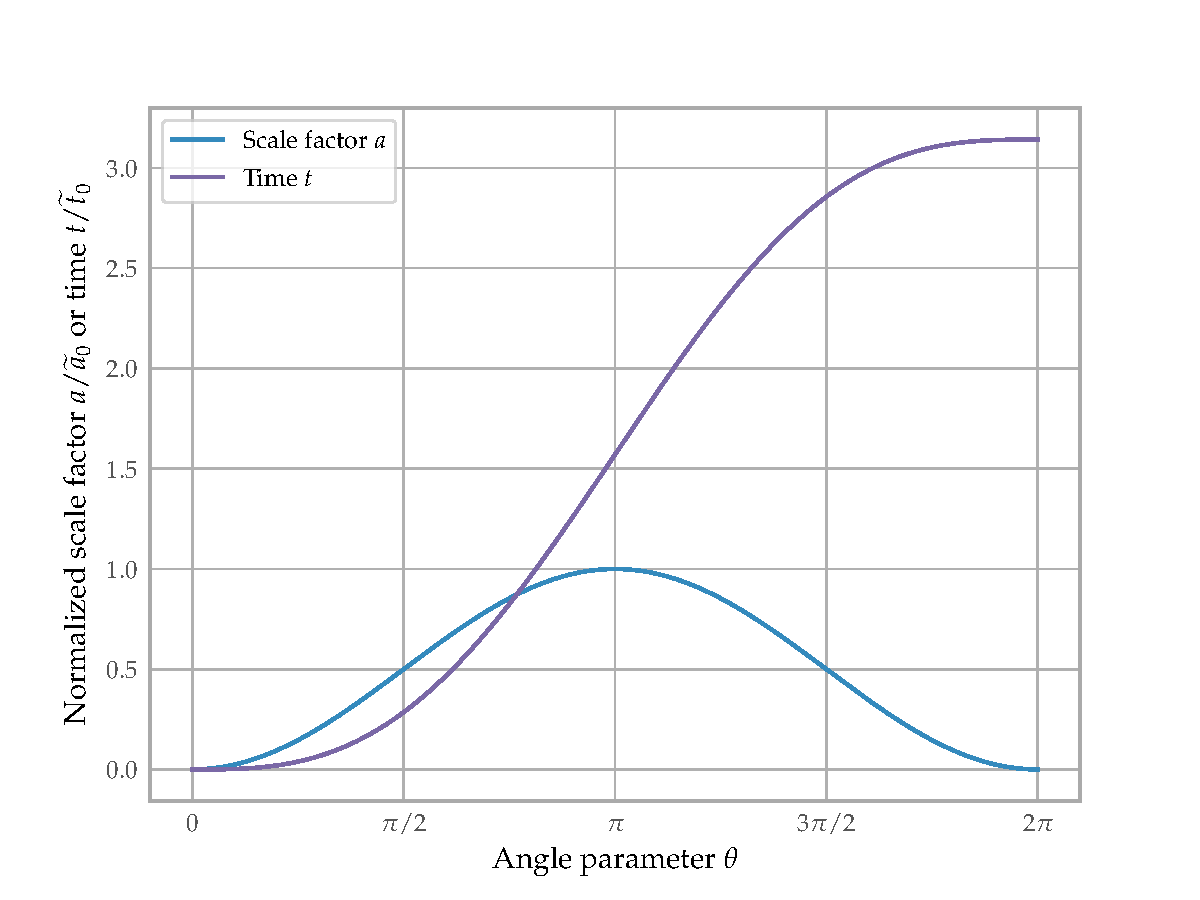
\includegraphics[width=\textwidth]{figures/positive_curvature_a.pdf}
\caption{A plot of \(a(\theta )\) and \(t(\theta )\).}
\label{fig:positive_curvature_a}
\end{figure}

We have \(\dot{a} > 0 \)   when \(0 \leq \theta \leq \theta_m = \pi \), while \(\dot{a} < 0\) when \(\theta _m \leq \theta \leq 2 \pi \): so, we call \(\theta_{m}\) the \emph{turn-around} angle.
The angles \(0\) and \(2 \pi \) correspond to the Big Bang and the Big Crunch.

At \(\theta _m\) we have: 
%
\begin{align}
  a_m &= \widetilde{a}_{0} =  a_0 \frac{\Omega_0}{\Omega_0 -1}  \\
  t_m &= \frac{\pi}{2} \widetilde{t}_0 = \frac{\pi}{2 H_0 } \frac{\Omega_0}{(\Omega_0 -1)^{3/2}}
\,.
\end{align}

\subsubsection{The age of a closed universe}

The total lifetime of the universe, in this scenario, is equal to \(2 t_m = \pi \widetilde{t}_{0}\). How does this compare to the result we found for a flat universe, namely \(t_0 = 2 / (3 H_0 )\) (equation \eqref{eq:einstein-de-sitter-age} with \(w=0\))?

We set \(a(t) = a_0 \), which means we are normalizing the scale factor to the current one: this yields 
%
\begin{align}
1= \frac{\Omega_0}{1-\Omega_0 } \frac{1 - \cos \theta }{2}
\qquad \implies \qquad
\cos \theta = 1 - \frac{2 (\Omega_0 -1)}{\Omega_0 } = \frac{2}{\Omega_0 }-1
\,,
\end{align}
%
so we can invert the cosine (assuming we are in the expanding phase: it is not invertible globally) and insert our expression for \(\theta \) into the expression for the time, to get\footnote{We need to use the expression \(\sin(
\arccos(x)) = \sqrt{1- \cos^2(\arccos x)} = \sqrt{1- x^2}\) with \(x = 2/ \Omega_0 -1\), and then the following manipulation: 
%
\begin{align}
\sqrt{1 - \qty(\frac{2}{\Omega_0 }-1)^2} = \sqrt{1 - \frac{4}{\Omega_0^2} + \frac{4}{\Omega_0} -1}
= \frac{2}{\Omega_0 } \sqrt{\Omega_0 -1 }
\,.
\end{align}}
%
\begin{equation} \label{eq:positive-curvature-age}
  t_0 = \frac{1}{2H_0 } \frac{\Omega_0  }{(\Omega_0 -1)^{3/2}} \qty(\arccos (\frac{2}{\Omega_0 }-1) - \frac{2}{\Omega_0 } \sqrt{\Omega_0 -1 })
\,.
\end{equation}

\begin{figure}[ht]
\centering
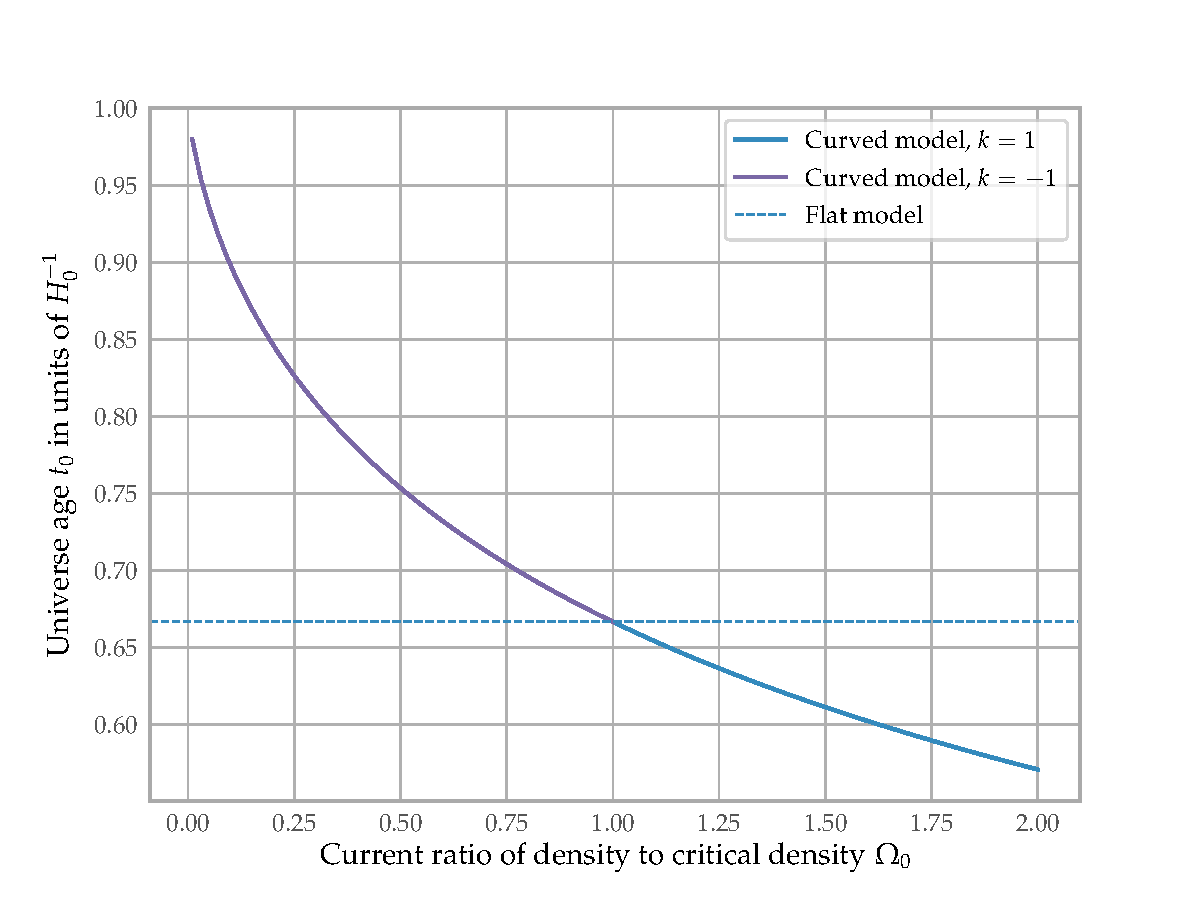
\includegraphics[width=\textwidth]{figures/curved_universe_age}
\caption{Universe age at the current time as a function of \(\Omega_0 \). For \(\Omega_0>1\) we use the positive curvature model in equation \eqref{eq:positive-curvature-age}: the age is lower than \(2/(3H_0 )\); for \(\Omega_0 <1\) we use the negative curvature model \eqref{eq:negative-curvature-age}: the age is greater than \(2/(3H_0 )\).
The flat model is plotted with a horizontal line for clarity, but if the universe is spatially flat then we must have \(\Omega_0 =1\).}
\label{fig:curved_universe_age}
\end{figure}

As we can see in figure \ref{fig:curved_universe_age}, this means that the estimated age of the universe is lower than \(2/(3H_0 ) \approx \SI{9.6}{Gyr}\), while the measured age of the universe is around \SI{14}{Gyr}.

\subsection{Negative curvature: an open universe}

For \(k = -1\) we do exactly the same steps with hyperbolic functions instead of trigonometric ones, calling the argument of these functions \(\psi \) instead of \(\theta \): we get 
%
\begin{align}
  a ( \psi ) &= a \frac{\Omega_0 }{2 (1-\Omega_0)} \qty(\cosh \psi -1) \\
  t (\psi ) &=  \frac{1}{H_0 } \frac{\Omega_0}{2 (\Omega_0 -1)^{3/2}}(\sinh \psi - \psi  )
\,,
\end{align}
%
and as before we can calculate the independent variable with \(\cosh\psi = 2/\Omega_0 -1\).\footnote{A doubt one might have: where does the sign change from \(\theta  - \sin(\theta )\) to \(\sinh(\psi ) - \psi \)? 

The difference between the calculations with the trigonometric functions and the hyperbolic functions lies in the substitution \(2 \theta = \pi - \alpha \): in the hyperbolic case we cannot do it this way, since the hyperbolic functions do not have any periodicity like this. Instead, the right substitution looks like \(2 \psi = i \pi + u\), since \(\sinh(i \pi + u) = -\sinh(u)\).

Then, we have the same expressions as before, but their sign is flipped.}

An analogous reasoning to the one before gives us 
%
\begin{align} \label{eq:negative-curvature-age}
t_0 = \frac{1}{2H_0 } \frac{\Omega_0}{(1-\Omega_0 )^{3/2}} \qty(\frac{2}{\Omega_0 } \sqrt{1 - \Omega_0 } - \operatorname{arccosh} \qty(\frac{2}{\Omega_0 } -1)) 
\marginnote{Now \(\sinh(\operatorname{arccossh}(x)) = \sqrt{x^2-1}\)}
\,,
\end{align}
%
which is plotted, again, in figure \ref{fig:curved_universe_age}: in this case \(t_0 > 2 / (3 H_0 )\)! This is then more attractive.

% \todo[inline]{In Pacciani's notes \cite[pag. 26]{Pacciani:2018} this is reported with an incorrect global sign.}

\subsection{Considerations on curvature}

The experimental fact that \(t_0 > 2/(3H_0 )\) seems to favour an open universe. 
However, the age of the universe is \(t_0 \approx \num{.96} H_0^{-1}\): looking at figure \ref{fig:curved_universe_age} it is clear that in order to account for it with spatial curvature only we would need \(\Omega_0 \ll 1\), and actually \(\Omega_0 < \Omega_{0m}\), where \(\Omega_{0m}\) is the current measured ratio of the density of matter to the critical density. 

In fact, in the current \(\Lambda \)CDM model of cosmology this is accounted for using dark energy, which means a positive cosmological constant.

From the second Friedmann equation 
%
\begin{align}
\frac{\ddot{a}}{a} =- \frac{4 \pi G}{3} \rho (1+3w) 
\,
\end{align}
%
we know that \(\ddot{a} < 0\), that is, the expansion of the universe decelerates if \(w > - 1/3\).
A singular instant at which \(a =0\) must be reached if \(w>-1/3\), while this is not necessarily the case for \(w<-1/3\).
As we will discuss in the next chapter, this will be one of the motivations behind the theory of inflation, which does not require the presence of an initial singularity. 

% \todo[inline]{Comment on inflationary theory}

\chapter{The thermal history of the universe}

In the study of the early stages of the universe the variation of the temperature, which determines the distribution of the energies of the collisions of the particles, plays a central role.
It makes sense to talk about temperature when the particles are actually in thermal equilibrium, as they were in the early universe: photons and electrons were continuously Compton-scattering off each other. 
After the particles stop continuously interacting we say that they \emph{decoupled}, and each component evolves independently. 

The fact that the universe's temperature was much higher in the past is need to explain \emph{primordial nucleosynthesis}: Helium-4 is the outcome of Hydrogen burning but in stellar evolution it is burned into heavier elements after it is formed, so we would expect to see small amounts of it. 
Instead, we see a relatively large amount of Helium-4: it makes up about a quarter of the universe by mass. 
The primordial universe being very hot helps account for this. 
In fact, this was first predicted in 1948, in the notorious \(\alpha \beta \gamma \) paper \cite[]{alpherOriginChemicalElements1948}. 

\section{Radiation energy density and the equality redshift}

In section \ref{sec:common-equations-of-state} we discussed the evolution of the energy density of matter and radiation, showing that for radiation \(\rho _r (z ) = \rho _{0r} (1+z)^{4}\) while for matter
\(\rho _m (z) = \rho_{0m} (1+z)^{3}\). 
We discussed this in the context of electromagnetic radiation, but it describes well the behavior of very relativistic particles, such as neutrinos. 

We can define a moment called the \emph{equality redshift} \(z _{\text{eq}}\).
This is when the energy density of radiation and that of matter were equal: \(\rho _r (z _{\text{eq}}) = \rho _m (z _{\text{eq}})\).
This means that 
%
\begin{equation}
\rho_{0,r} (1+z _{\text{eq}})^{4} = \rho_{0,m} (1+z _{\text{eq}})^{3} \implies
(1+z _{\text{eq}}) = \frac{\rho _{0,m}}{\rho _{0,r}} 
  = \frac{\Omega_{0,m}}{\Omega_{0,r}}
\,,
\end{equation}
%
where we divided and multiplied by the critical density today. 

We know that \(\Omega_{0,m}\) is around \num{0.3}, while for the radiation we can deduce the density from the spectrum of the CMB.

Accounting for everything, we think that 
%
\begin{equation}
  1 + z _{\text{eq}} \simeq \num{2.3e4} \Omega_{0, m} h^2
  \approx 3370
\,.
\end{equation}

The value is that obtained from the Planck Collaboration \cite[]{PlanckCollaboration:2016XIII}.

This means that the recombination of electrons and protons into Hydrogen, which occurred around redshift \(z _{\text{CMB}} \approx 1090\), happened when the universe was already \emph{matter dominated} --- specifically, the density of matter was \(\approx 3\) times that of radiation.

Another interesting time is \(z_\Lambda \), when the energy density due to the cosmological constant equalled that of matter:  \(\rho _m (z_{\Lambda }) = \rho _\Lambda (z_\Lambda )\), which is calculated with the same reasoning as \(z _{\text{eq}}\), recalling that \(\rho_{\Lambda }\) is a constant with respect to the redshift:
\begin{equation}
1+ z_\Lambda = \qty(\frac{\rho_{0, \Lambda }}{\rho_{0,m}})^{1/3} \simeq \qty(\frac{0.7}{0.3})^{1/3} \approx \num{0.33}
\,.
\end{equation}

This is relatively close, in cosmological terms: the comoving distance corresponding to this redshift is around \SI{1350}{Mpc}, less than \SI{10}{\percent} of the comoving distance to the CMB. 

% The model which won out is the \emph{hot Big Bang} model.

What is the temperature of a radiation-dominated universe?
From the Stefan-Boltzmann law we know that \(\rho _r \propto T^{4}\), while as we have discussed previously \(\rho _r \propto a^{-4}\).
Therefore, we expect \(T \propto 1/a\) to hold: this is known as \emph{Tolman's law}.
In this chapter we will discuss how this does approximately hold, but we need to make some corrections due to the annihilation of ultrarelativistic particles.

We know that in a radiation dominated universe \(a \propto t^{1/2}\), which means that \(T \propto t^{-1/2}\).

We shall describe the pressure \(P\), number density \(n\) and energy density \(\rho  \) in the universe, as functions of the chemical potentials \(\mu \) and of  the temperature \(T\).
We will use natural units, so that \(c= \hbar = k_B = 1\): so, temperatures and masses will be measured in electronVolts. 

This is very convenient, since it allows us to make the following consideration: when the temperature will be of the order of the mass of a certain elementary particle, then statistically that type of particle will usually be ultra-relativistic.

This section will mostly follow Weinberg's book \cite[page 538, section 15.6]{weinbergGravitationCosmologyPrinciples1972}.

\section{Thermodynamics in the early universe}

We will express the quantities mentioned above: \(P\), \(\rho \) and \(n\) in terms of the distribution of particles in phase space: in general the phase space for a single particle in 3D is six-dimensional, but we operate under the assumption that the cosmological principle holds, so by homogeneity the spatial dependence of the distribution function can be neglected. 
Thus, we can talk of densities\footnote{As a general rule, one should avoid talking about ``global quantities'': the universe is, in principle, infinite, we should refer at most to what is or could be inside our light cone. It is better to work in terms of densities.}, neglecting the spatial position, and integrating over momentum space to gather all the information there is to know about the particles in that position.

\subsection{Number density, energy density and pressure}

\subsubsection{Number density}

If \(f(\vec{q})\) is the distribution density of particles with three-dimensional momentum \(\vec{q}\), the number density of particles is given by: 
%
\begin{equation}\label{eq:number-density-momentum-space}
  n = \frac{g}{(2 \pi )^3} \int \dd[3]{q} f(\vec{q}, T, \mu )
\,,
\end{equation}
%
where the parameter \(g\) is the number of helicity states: it is the number of particles we can have with different quantum numbers, after fixing momentum and position. 

This essentially is our choice for the normalization of the distribution function. 
We include the factor \((2\pi)^3 \) in order to normalize the integral: the number of particles, a pure number, is given by
%
\begin{align}
N \propto \int \dd[3]{q} \dd[3]{x}  f(\vec{q}, \vec{x})
\,,
\end{align}
%
so the right hand side's differentials have the dimensions of an action cubed: we need to normalize them, and the conventional action used to do so is \(h = 2 \pi \hbar\).
So, when we set \(\hbar = 1\) we get a factor \((2\pi )^3\) on the denominator. 
Do note that the \(\dd[3]{x}\) integral, giving a volume, is brought to the left in our expression to give a number density. 

\subsubsection{The number of helicity states}

The only quantum number which can vary after fixing those if we are considering an elementary particle is the spin component \(s_z\); therefore if the total spin is \(s\) we should have \(2s+1\) possible spin states.
For example  electrons, which have spin \(1/2\), will have \(g = 2s+1 = 2\). 

% We will have to integrate  over position and momentum: the metric we will get in the end must not depend on anything but time, by the cosmological principle.

Things, however, are more complicated than this: for photons, we only have two spin states (\(g=2\)) even though they have \(s=1\), since \(s_z=0\) is unphysical for a photon. 
Gravitons also have \(g=2\) even though their total spin is \(s=2\): this is because \(\abs{s_z} \leq 1 \) is unphysical for a graviton. 
In general for massless particles Lorentz invariance guarantees the fact that transverse modes cannot exist, since we cannot go in the rest frame of the particle.\footnote{Some more details on this: if we measure the spin component \(s_z\) to be equal to some value in a certain reference frame, then this will mean: (1) if \(s_z \neq 0 \) we need a rotation of at least \(2 \pi / s_z\) around the \(z\) axis in order to recover the system we started with, while (2) if \(s_z=0\) the system is symmetric with respect to rotations around the \(z\) axis. 

So, for a photon to have \(s_z=0\) we would need to be in a frame in which its wavefunction was cylindrically symmetric. This cannot be the case if the photon is travelling in the \(z\) direction, so we must be in the rest frame of the photon, which does not exist. 

Similarly, for gravitons the argument as to why \(s_z \neq 0\) still applies, and we can exclude the spins \(\abs{s_z} = 1\) by the following argument: in full generality we can remove all the gauge freedom in a gravitational wave by going to TT gauge, and we can show that in TT gauge the wave is symmetric under rotations of angle \(\pi \) about the \(z\) axis. 
Therefore, the spin of the graviton must be at least \(2\) in magnitude.}

Even for massive particles we do not always have \(g = 2s+1\): \(g\) accounts for all internal degrees of freedom, and as the temperature drops below a certain value we need to consider composite particles as well: for atoms we also have vibration, rotation and such. These all contribute to \(g\). 

\subsubsection{Energy density}

The energy density is given by
%
\begin{equation} \label{eq:energy-density-momentum-space}
  \rho = \frac{g}{(2 \pi )^3} \int \dd[3]{q} E(q) f(\vec{q}, T, \mu ) 
\,,
\end{equation}
%
where \(E^2 = q^2 + m^2\)\footnote{Particles are on-shell, that is they obey the equations of motion (which is not mandatory, and this is what Quantum Mechanics is all about).}.
For photons \(E = q\), for nonrelativistic particles \(E \approx m + q^2 / 2m\).
Here we are denoting the modulus of the momentum vector as \(q = \abs{\vec{q}}\). 

This formula is a weighted average of the energies on the distribution function on the momenta. 

\subsubsection{Pressure}

The adiabatic pressure is 
%
\begin{equation}\label{eq:pressure-momentum-space}
  P = \frac{g}{(2 \pi )^3} \int \dd[3]{q} \frac{q^2 f(\vec{q}, T, \mu )}{3E(q)} 
\,.
\end{equation}

\begin{bluebox}  
This comes from a consideration of the diagonal components of the stress energy tensor of an ideal fluid: we know that 
%
\begin{align}
T^{\mu \nu }
= \left[\begin{array}{cccc}
\rho  & 0 & 0 & 0 \\ 
0 & P & 0 & 0 \\ 
0 & 0 & P & 0 \\ 
0 & 0 & 0 & P
\end{array}\right]
= \frac{g}{(2\pi )^3} \expval{ \int \frac{\dd[3]{q}}{E(\vec{q})} f(\vec{q}) p^{\mu } (\vec{q}) p^{\nu } (\vec{q})}
\,,
\end{align}
%
where \(p^{\mu } = (E(q), \vec{q})\) is the momentum vector.
Although it may not look like it, this formula is covariant.\footnote{we are integrating a tensorial expression (\(f p^{\mu } p^{\nu }\) is a tensor) with respect to a covariant integration element: \(\dd[3]{q} / E(q)\) is a scalar with respect to Lorentz transformations, since it can be obtained as 
%
\begin{align}
\dd[4]{q} \delta (E^2 - p^2 - m^2) = \frac{ \dd[3]{q}}{2E} \delta (E - \sqrt{m^2+p^2})
\,.
\end{align}
}
The average sign is meant to indicate a spatial average, across volumes which are wide enough for homogeneity to hold. 

This formula reproduces equation \eqref{eq:energy-density-momentum-space} for \(\mu = \nu = 0\): indeed, in this case \(p^{0} (q) = E(q)\).
The off-diagonal components are zero by isotropy: if they were not, we would see heat and particle flow in specific directions. 

So, for the diagonal components spatial components the integrand looks like \(q^{i} q^{j} / E(q)\). 

The formula for the pressure then follows by isotropy: the total force per unit area to go around is \(q^2 / E\), and it must be distributed equally in the three spatial directions, so if we want to switch from the directional integral \(T^{ii} = P \propto \int q^{i} q^{i} / E\) (not summed over \(i\)) to an integral of the modulus of the momentum, \(P \propto \int q^2 / E\) we must divide by 3. 
\end{bluebox}


% Alternatively, we can say that this comes from imposing \(\dd{E} = P \dd{V} + \dd{Q} \).

This definition gives us \(P = \rho /3\) for photons directly, which can be seen by substituting \(E = q\). 

\subsubsection{The distribution function}

If the particles are in thermal equilibrium, the distribution in momentum space will be given by the following expression: 
%
\begin{equation}
  f(\vec{q}) = \qty(\exp(\frac{E(q)- \mu }{T}) \pm 1 )^{-1}
\,,
\end{equation}
%
where we have a plus for fermions, and a minus for bosons. Here, \(\mu = \pdv*{\rho }{n}\) is the chemical potential, the derivative of the energy (density) with respect to a change in the number (density) of particles: is becomes relevant when the gas becomes hot and dense, if it is sparse then adding particles does not affect the energy.

% It can be introduced as a Lagrange multiplier for changes in number of particles.

The Planck distribution, which describes the statistics of photons, is consistent with this, since it is given by: 
%
\begin{equation}
  f_k(\vec{q}) = \qty(\exp(\frac{q}{T}) -1 )^{-1}
\,,
\end{equation}
%
since they are bosons with no chemical potential.\footnote{This seemed weird to me: is the Planck function not 
%
\begin{align}
B_{\nu } (T) = \frac{2\nu^3}{e^{ 2 \pi \nu / T} -1 }
\,
\end{align}
%
in natural units? Well, these two are actually equivalent formulations. To see this, recall that in natural units \(q = E = \omega = 2 \pi \nu \) for a photon. First of all, they describe different physical quantities: the Planck function describes the \emph{spectral radiance}, \(\dd{E} = B_\nu (T) \dd{t} \dd{A} \dd{\nu } \dd{\Omega }\), while the distribution \(f(q)\) describes the number of particles per unit momentum volume: \(\dd{N} = f(q) \dd[3]{q}\).  

To check their equivalence, let us compute the energy density with both: 
%
\begin{align}
\rho &=  \frac{g}{(2\pi )^3} \int \frac{q}{e^{q/T}-1} \dd{\Omega } q^2 \dd{q} = \frac{2}{(2\pi )^3}\int \frac{ \omega^3}{e^{q/T}-1} \dd{\Omega } \dd{q}  
= \int \frac{2 \nu^3}{e^{2 \pi \nu /T}} \dd{\Omega } \dd{q}
\\
\text{but also}\quad\rho &= \dv{E}{V} = \int \frac{ \dd{E}}{ \dd{t} \dd{A} \dd{q} \dd{\Omega }} \dd{q} \dd{\Omega } = \int B_q(T) \dd{\Omega } \dd{q}
\,,
\end{align}
%
where we used the fact that, in natural units \(\dd{V} = \dd{t} \dd{A}\).
}
The fact that the distribution of photons is indeed described by this distribution with \(\mu =0\) is a way to experimentally determine the fact that the chemical potential of photons is indeed zero. If we observed the distribution for physical blackbodies to have \(\mu \neq 0\) this would be called a \emph{spectral distortion}. The CMB is wonderfully consistent with \(\mu =0\), it is actually the best Planckian in Nature.

It is a fact that the chemical potential \(\mu \) can be neglected when dealing with the early universe. Let us justify this.

In general we can say that if for some chemical species we have the reaction \(i+j \leftrightarrow k+l\), and we reach chemical equilibrium, then the chemical potentials of the species will be connected by \(\mu _i + \mu _j = \mu _k + \mu _l\): this is called the \emph{Saha equation}.

Assuming that we are in thermal equilibrium is not in general valid, we we will do so in our discussion for simplicity, but non-equilibrium dynamics must be considered when dealing with CMB anisotropies.

By enumerating all the possible chemical reactions between the various particle types we will get a system of equations for their chemical potentials, complemented with some known facts, such as the fact that photons have \(\mu_{\gamma }=0\), which is the case since the photons do not interact with each other.

For example, from the annihilation of electron and positron \(e^{+}+ e^{-} \leftrightarrow 2 \gamma \) we can derive \(\mu _{e^{+}} = - \mu_{e^{-}}\).

% This rule is not trivial; it is an ansatz of thermodynamical equilibrium to get a solution of the Boltzmann equation which allows us to write the Saha equations.

\end{document}